\documentclass[a4paper, twocolumn]{article}
\usepackage[utf8]{inputenc}
\usepackage{amsmath}
\usepackage{graphicx}
\graphicspath{documents/}
\usepackage{caption}
\captionsetup{font=scriptsize}
\usepackage[margin=0.5in]{geometry}

\title{Atomic Spectroscopy}
\author{
Garcia, Jorge A.\\
\and
Lane, Ryan C. \\
\and
Miller, Patrick C.
}
\date{February 14th, 2018\\\line(1,0){500}}

\begin{document}
\maketitle

\section{Purpose}
The purpose of this experiment is to demonstrate the emission lines of the electromagnetic spectrum for different elements.
Diffraction is the key physical concept in this experiment, since an element will emit light it's light as a combination of
its different spectral lines, and it must be diffracted into its components in order to observe them individually. The only
controled quantity is that of the diffraction grating, while measured quantities during the experiment are that of the 
angles at which emission lines are seen. From these quantities, the wavelength of said emission lines will be determined and
an approximation of the Rydberg constant can be achieved.

\section{Apparatus and Method}


\section{Procedure}
The procedure was replicated for three different samples. After setting the discharge tube in front of the slit, it is important
to align the telescope to the center of the telescope pivot, so it is perpendicular to the parallel beam. This allows for the 
identification of the central emission line, which will be used as the reference point to find the rest of the lines. The telescope
will then be moved to find a new line, and recording of the angle indicated on the base is necessary. This measured angle has
at the very least an uncertainty of 0.1 degrees from pure instrumental limitations.

The first run was done with Mercury for calibration purposes and ensuring proper use of the equipment, as the tube has a longer
lifetime than that of Hydrogen. Hydrogen will be used to approximate the Rydberg constant. Finally, the spectrum of an unknown source
will be used, with the objective of identifying it.

\section{Data and Uncertainties}
Each member in the team did 2 sets of measurements, one for the left-side lines and another for the right-side. The angle at which
the undiffracted light is seen was not set to 0 degrees, and such all measurements were shifted, so only the change in angle from the center
line is taken into account. The 6 measurements for each of the lines are then averaged, in order to reach a mean value for the angle at which
the color is observed. The standard deviation of the mean is then:
\begin{equation}
 \Delta\theta = \sqrt{\frac{1}{N-1} \sum_{i=1}^{N}(\theta_i-\bar{\theta})^2}
\end{equation}

With N being the number of measurements, $\theta_i$ the ith measurement for an angle, and $\bar{theta}$ the mean value of that angle.
Calculation of the mean and error of the angles for each emission line was done in Python.

Shown in Table \ref{table:anglesHg} is the average measurements for the Mercury discharge tube. The uncertainty in the mean of each of the angles was
lower than 0.1 degrees, so our uncertainty in these measurements must be intrument dominated. 
\begin{table}[h!]
\centering
\begin{tabular}{ |c||c|c|c| }
 \hline
 \multicolumn{4}{|c|}{\textbf{Mercury (Hg)}} \\
 \hline
 \multicolumn{2}{|c}{\textbf{Degree Shift:}} &
 \multicolumn{2}{|c|}{139.4} \\
 \hline
 \textbf{Color} & $\boldsymbol{\theta}$ & $\boldsymbol{\Delta\theta}$ & \textbf{Order} \\
 \hline
 Violet & 15.1 & 0.1 & First \\
 \hline
 Green & 19.2 & 0.1 & First\\ 
 \hline
 Yellow & 20.3 & 0.1 & First \\
 \hline
 Orange & 20.4 & 0.1 & First \\
 \hline
\end{tabular}
\caption{Average Measurements for Hg}
\label{table:anglesHg}
\end{table}

For the measurements of Hydrogen emission lines (Table \ref{table:anglesH}), the human error was larger than for the 
previous measurements. This is possibly due to the lower intensity of the emission lines, making them harder to be seen.
Another detail with this discharge tube is the sudden appearance of a blue emission line, which hadn't been seen near
the Cyan line. This means this linedax
\begin{table}[h!]
\centering
\begin{tabular}{ |c||c|c|c| }
 \hline
 \multicolumn{4}{|c|}{\textbf{Hydrogen (H)}} \\
 \hline
 \multicolumn{2}{|c}{\textbf{Degree Shift:}} &
 \multicolumn{2}{|c|}{139.4} \\
 \hline
 \textbf{Color} & $\boldsymbol{\theta}$ & $\boldsymbol{\Delta\theta}$ & \textbf{Order} \\
 \hline
 Violet & 15.1 & 0.1 & First \\
 \hline
 Cyan & 17.0 & 0.2 & First \\ 
 \hline
 Red & 23.3 & 0.2 & First \\
 \hline
 Blue & 35.75 & 0.3 & Second \\
 \hline
\end{tabular}
\caption{Average Measurements for H}
\label{table:anglesH}
\end{table}

The most problems occured with the Unknown Sample A. The emission lines were too faint to be accurately measured, even after
attempts of darkening the room. Because of these difficulties and lack of time to take more measurements, our data is very
imprecise. This especially can be seen in the last two angles.
\begin{table}[h!]
\centering
\begin{tabular}{ |c||c|c|c| }
 \hline
 \multicolumn{4}{|c|}{\textbf{Unknown Sample A}} \\
 \hline
 \multicolumn{2}{|c}{\textbf{Degree Shift:}} &
 \multicolumn{2}{|c|}{139.4} \\
 \hline
 \textbf{Color} & $\boldsymbol{\theta}$ & $\boldsymbol{\Delta\theta}$ & \textbf{Order} \\
 \hline
 1 & 14.4 & 0.2 & First \\
 \hline
 2 & 14.4 & 0.3 & First \\
 \hline
 3 & 15.5 & 0.1 & First \\
 \hline
 4 & 17.7 & 2.1 & First \\
 \hline
 5 & 23.2 & 5.3 & First \\
 \hline
\end{tabular}
\caption{Average Measurements for Unknown Sample A}
\label{table:anglesA}
\end{table}

\section{Analysis and Uncertainties}
Knowing the angle at which an emission line is seen, and given the spacing of the diffraction grating lines, the
wavelengths can be calculated as:
\begin{equation*}
 dsin\theta = m\lambda
\end{equation*}
\begin{equation}
 \lambda = \frac{dsin\theta}{m}
\end{equation}
Accordingly, when calculating the wavelength, the error from the angle of the emission line propagates as follows:
\begin{equation}
 \Delta\lambda = \frac{1}{m} \sqrt{ sin^2\theta (\Delta d)^2 + d^2 cos^2\theta (\Delta\theta)^2 }
\end{equation}

The results were then calculated in Python using Equations 2 and 3.

\begin{table}[h!]
\centering
\begin{tabular}{ |c||c|c| }
 \hline
 \multicolumn{3}{|c|}{\textbf{Mercury (Hg)}} \\
 \hline
 \textbf{Color} & $\boldsymbol{\lambda}$ $(nm)$ & $\boldsymbol{\Delta\lambda}$ $(nm)$ \\
 \hline
 Violet & 434.6 & 2.8 \\
 \hline
 Green & 548.6 & 2.7 \\ 
 \hline
 Yellow & 577.8 & 2.7 \\
 \hline
 Orange & 581.4 & 2.7 \\
 \hline
\end{tabular}
\caption{Determined wavelengths and $sin\theta$ for Hg}
\label{table:lambdaHg}
\end{table}

\begin{figure}[h!]
 \centering
 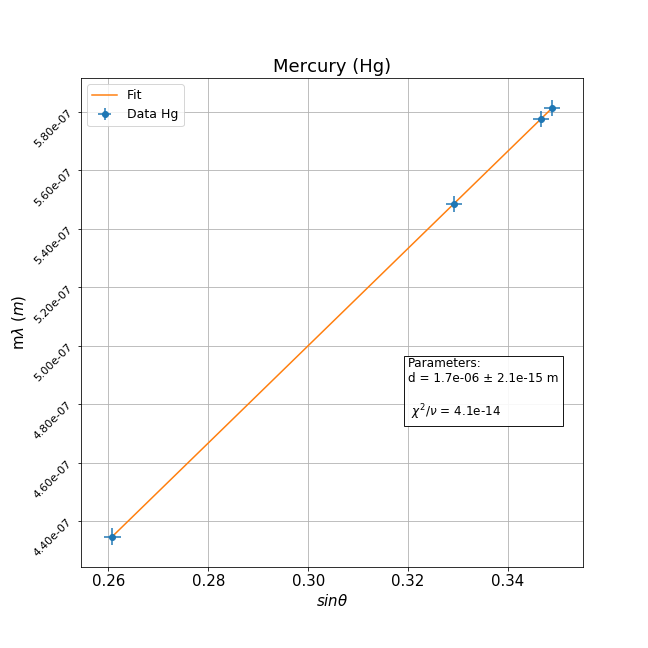
\includegraphics[scale = 0.4]{mercury}
 \caption{Plot of Mercury's $sin\theta$ against $m\lambda$}
 \label{fig:mercury}
\end{figure}

\begin{table}[h!]
\centering
\begin{tabular}{ |c||c|c| }
 \hline
 \multicolumn{3}{|c|}{\textbf{Hydrogen (H)}} \\
 \hline
 \textbf{Color} & $\boldsymbol{\lambda}$ $(nm)$ & $\boldsymbol{\Delta\lambda}$ $(nm)$ \\
 \hline
 Violet & 435.1 & 3.5 \\
 \hline
 Blue & 486.8 & 3.1 \\
 \hline
 Cyan & 487.3 & 4.8 \\ 
 \hline
 Red & 657.9 & 4.0 \\
 \hline
\end{tabular}
\caption{Determined wavelengths for H}
\label{table:lambdaH}
\end{table}

\begin{table}[h!]
\centering
\begin{tabular}{ |c|c|c|c|c|c| }
 \hline
 \multicolumn{6}{|c|}{\textbf{Hydrogen Balmer Series}} \\
 \hline
  & \multicolumn{5}{|c|}{$\boldsymbol{n_i}$} \\
 \hline
  & & 3 & 4 & 5 & 6 \\
 \hline
 $\boldsymbol{n_f}$ & 2 & 32 & 42 & 52 & 62 \\
 \hline
\end{tabular}
\caption{Expected wavelengths for electron transitions of H}
\label{table:lambdaH}
\end{table}

\begin{figure}[h!]
 \centering
 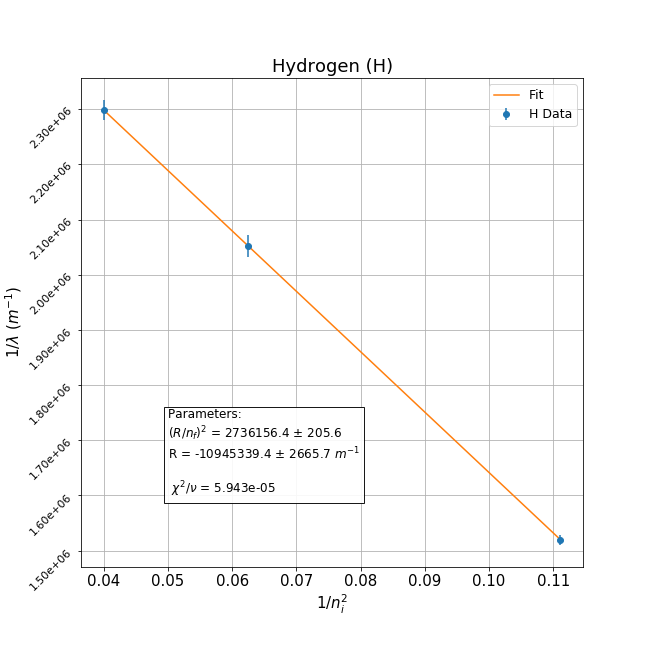
\includegraphics[scale = 0.4]{hydrogen}
 \caption{Plot of Hydrogen's $\frac{1}{n^2}$ against $\frac{1}{\lambda}$}
 \label{fig:hydrogen}
\end{figure}

\begin{table}[h!]
\centering
\begin{tabular}{ |c||c|c| }
 \hline
 \multicolumn{3}{|c|}{\textbf{Unknown Sample A}} \\
 \hline
 \textbf{Color} & $\boldsymbol{\lambda}$ $(nm)$ & $\boldsymbol{\Delta\lambda}$ $(nm)$ \\
 \hline
 1 & 415.9 & 4.2 \\
 \hline
 2 & 415.9 & 7.0 \\
 \hline
 3 & 445.4 & 3.2 \\
 \hline
 4 & 506.7 & 5.8 \\
 \hline
 5 & 655.2 & 1.2 \\
 \hline
\end{tabular}
\caption{Determined wavelengths for Unknown Sample A}
\label{table:lambdaA}
\end{table}

\section{Results}


\section{Conclusions}


\end{document}